\documentclass[12pt,letterpaper]{article}
\usepackage{graphicx,textcomp}
\usepackage{natbib}
\usepackage{setspace}
\usepackage{fullpage}
\usepackage{color}
\usepackage[reqno]{amsmath}
\usepackage{amsthm}
\usepackage{fancyvrb}
\usepackage{amssymb,enumerate}
\usepackage[all]{xy}
\usepackage{endnotes}
\usepackage{lscape}
\newtheorem{com}{Comment}
\usepackage{float}
\usepackage{hyperref}
\newtheorem{lem} {Lemma}
\newtheorem{prop}{Proposition}
\newtheorem{thm}{Theorem}
\newtheorem{defn}{Definition}
\newtheorem{cor}{Corollary}
\newtheorem{obs}{Observation}
\usepackage[compact]{titlesec}
\usepackage{dcolumn}
\usepackage{tikz}
\usetikzlibrary{arrows}
\usepackage{multirow}
\usepackage{xcolor}
\newcolumntype{.}{D{.}{.}{-1}}
\newcolumntype{d}[1]{D{.}{.}{#1}}
\definecolor{light-gray}{gray}{0.65}
\usepackage{url}
\usepackage{listings}
\usepackage{color}

\definecolor{codegreen}{rgb}{0,0.6,0}
\definecolor{codegray}{rgb}{0.5,0.5,0.5}
\definecolor{codepurple}{rgb}{0.58,0,0.82}
\definecolor{backcolour}{rgb}{0.95,0.95,0.92}

\lstdefinestyle{mystyle}{
	backgroundcolor=\color{backcolour},   
	commentstyle=\color{codegreen},
	keywordstyle=\color{magenta},
	numberstyle=\tiny\color{codegray},
	stringstyle=\color{codepurple},
	basicstyle=\footnotesize,
	breakatwhitespace=false,         
	breaklines=true,                 
	captionpos=b,                    
	keepspaces=true,                 
	numbers=left,                    
	numbersep=5pt,                  
	showspaces=false,                
	showstringspaces=false,
	showtabs=false,                  
	tabsize=2
}
\lstset{style=mystyle}
\newcommand{\Sref}[1]{Section~\ref{#1}}
\newtheorem{hyp}{Hypothesis}

\title{Problem Set 3}
\date{Due: November 12, 2021}
\author{Applied Stats/Quant Methods 1}


\begin{document}
	\maketitle
	\section*{Instructions}
	\begin{itemize}
		\item Please show your work! You may lose points by simply writing in the answer. If the problem requires you to execute commands in \texttt{R}, please include the code you used to get your answers. Please also include the \texttt{.R} file that contains your code. If you are not sure if work needs to be shown for a particular problem, please ask.
		\item Your homework should be submitted electronically on GitHub in \texttt{.pdf} form.
		\item This problem set is due before class on Friday November 12, 2021. No late assignments will be accepted.
		\item Total available points for this homework is 80.
	\end{itemize}

	
		\vspace{.25cm}
	
\noindent In this problem set, you will run several regressions and create an add variable plot (see the lecture slides) in \texttt{R} using the \texttt{incumbents\_subset.csv} dataset. Include all of your code.

	\vspace{.5cm}
\section*{Question 1} %(20 points)}
\vspace{.25cm}
\noindent We are interested in knowing how the difference in campaign spending between incumbent and challenger affects the incumbent's vote share. 
	\begin{enumerate}
		\item Run a regression where the outcome variable is \texttt{voteshare} and the explanatory variable is \texttt{difflog}.	\vspace{5cm}
		
		
		\begin{lstlisting}[language=R]
		
		# 1. run a regression where the outcome variable is 'voteshare' and the explanatory variable is 'difflog'
# voteshare - outcome variable is the 'dependent variable on Y'

# difflog - explanatory variable is the 'independent variable (predictor variable) on X' 
# unknown parameter θ
# the basic prediction equation expresses a linear relationship between an independent variable 
# or (x, predictor variable) and a dependent variable (y, a criterian variable)

incumbents <- read.csv("https://raw.githubusercontent.com/ASDS-TCD/StatsI_Fall2021/main/datasets/incumbents_subset.csv")
summary(incumbents) # this is a simple regression or summary(..)
str(incumbents)
attach(incumbents)
names(incumbents)


# difflog depends on voteshare ..
# q1 <- lm(difflog ~ voteshare, data = incumbents)
# summary(q1)
q1 <- lm(voteshare ~ difflog, data = incumbents)
summary(q1)

plot(difflog ~ voteshare, data = incumbents)
abline(lm(difflog ~ voteshare, data = incumbents), col = "blue")
		
		\end{lstlisting}
		
		\item Make a scatterplot of the two variables and add the regression line. 	\vspace{7cm}
		
		\begin{lstlisting}[language=R]
		
		### 2. Make a scatterplot of the two variables and add the regression line ####

# the ggplot plots the regression line
#q1_plot <- ggplot(incumbents, aes(difflog, voteshare)) +
  # geom_point(alpha = 0.5) + # add a scatterplot
#  geom_smooth(method = "lm") # add a linear regression line
# run the plot
#q1_plot

class(voteshare)
class(difflog)
plot(difflog, voteshare, main = "Scatterplot")
cor(difflog, voteshare) # x,y

# testing the incumbents_subset dataset
# scatter.smooth(x=incumbents$difflog, y=incumbents$voteshare, main="Scatter") 

# the ggplot plots the regression
q1_plot <- ggplot(incumbents, aes(difflog, voteshare)) +
  geom_point(alpha = 0.5) + # add a scatterplot
  geom_smooth(method = "lm") + # add a linear regression line
  labs(x = "difflog", y = "voteshare")
q1_plot

# using the lm() function for plotting the output

summary(lm(data = incumbents, difflog~ voteshare))
		
		\end{lstlisting}
		
		
		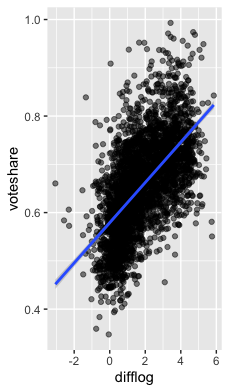
\includegraphics[scale=0.85]{plot_1.png}
		
		\item Save the residuals of the model in a separate object.	\vspace{7cm}
		
		
		\begin{lstlisting}[language=R]
		
		### 3. Save the residuals of the model in a separate object

# plotting the residuals

q1_resid <- resid(q1) #a function for extracting the residuals from
#a model object
plot(incumbents$difflog, q1_resid)
abline(h = 0, col = "red")

q1resid <- q1$residuals
q1resid 

q1_resid <- resid(q1) #a function for extracting the residuals from
#a model object
plot(incumbents$voteshare, q1_resid)
abline(h = 0, col = "red")
		
		
		\end{lstlisting}
		
		\item Write the prediction equation.
		
		\begin{lstlisting}[language=R]
		
# (Intercept) 0.579031 and difflog  0.041666 (from the summary)
# x is the difference for challenger's spending
 # y (hat) = 0.579031 + 0.041666x 
 
		
			\end{lstlisting}

(Intercept) 0.579031 and difflog  0.041666 is from summary(q1)
x is the difference for challenger's spending

$\hat{y}$	= 0.579031 + 0.041666x 	
		
	\end{enumerate}
	
\newpage

\section*{Question 2}% (20 points)}
\noindent We are interested in knowing how the difference between incumbent and challenger's spending and the vote share of the presidential candidate of the incumbent's party are related.	\vspace{.25cm}
	\begin{enumerate}
		\item Run a regression where the outcome variable is \texttt{presvote} and the explanatory variable is \texttt{difflog}.	\vspace{5cm}
		
		\begin{lstlisting}[language=R]
		
		## 1. Run a regression where the outcome variable is 'prevote' and the explanatory variable
# is 'difflog' 

# 'prevote' is the dependent variable (outcome variable) on Y axis
# ' difflog' is the independent variable (explanatory variable) on X axis
		
		q2 <- lm(presvote ~ difflog, data = incumbents)
summary(q2)
plot(difflog ~ presvote, data = incumbents)
abline(lm(difflog ~ presvote, data = incumbents), col = "blue")
		
		\end{lstlisting}
		
		
		\item Make a scatterplot of the two variables and add the regression line. 	\vspace{5cm}
		
		\begin{lstlisting}[language=R]
		
## 2. Make a scatterplot of the two variables and add the regression line

# the ggplot plots the regression
q2_plot <- ggplot(incumbents, aes(difflog, presvote)) +
  geom_point(alpha = 0.5) + # add a scatterplot
  geom_smooth(method = "lm") + # add a linear regression line
  labs(x = "difflog", y = "presvote")
q2_plot
		
		\end{lstlisting}
		
		
		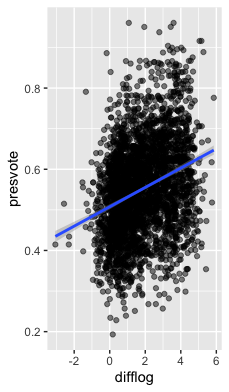
\includegraphics[scale=0.85]{plot_2.png}
		
		\item Save the residuals of the model in a separate object.	\vspace{5cm}
		
		
		\begin{lstlisting}[language=R]
		
		## 3. Save the residuals of the model in a separate object.

q2_resid <- resid(q2) #a function for extracting the residuals from
#a model object
plot(incumbents$voteshare, q2_resid)
abline(h = 0, col = "red")

q2resid <- q2$residuals
q2resid
		
		\end{lstlisting}
		
		
		\item Write the prediction equation.
		
		(Intercept) 0.507583 and difflog  0.023837 is from summary(q2)


$\hat{y}$	= 0.507583 + 0.023837x	
		
	\end{enumerate}
	
	\newpage	
\section*{Question 3}% (20 points)}

\noindent We are interested in knowing how the vote share of the presidential candidate of the incumbent's party is associated with the incumbent's electoral success.
	\vspace{.25cm}
	\begin{enumerate}
		\item Run a regression where the outcome variable is \texttt{voteshare} and the explanatory variable is \texttt{presvote}.
		
		
		\begin{lstlisting}[language=R]
		
		# 1. Run a regression where the outcome variable is 'voteshare' and the explanatory varaible'
# is 'presvote'

q3 <- lm(voteshare ~ presvote, data = incumbents)
summary(q3)
plot(presvote ~ voteshare, data = incumbents)
abline(lm(presvote ~ voteshare, data = incumbents), col = "blue")
		
		
		\end{lstlisting}
		
		
			\vspace{5cm}
		\item Make a scatterplot of the two variables and add the regression line. 
		
		
		\begin{lstlisting}[language=R]
		
		
		# ## 2. Make a scatterplot of the two variables and add the regression line

# the ggplot plots the regression
q3_plot <- ggplot(incumbents, aes(presvote, voteshare)) +
  geom_point(alpha = 0.5) + # add a scatterplot
  geom_smooth(method = "lm") # add a linear regression line
q3_plot
		
			\end{lstlisting}
			
			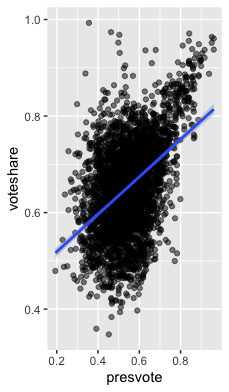
\includegraphics[scale=0.85]{plot_3.png}
		
			\vspace{5cm}
		\item Write the prediction equation.
		
		
				(Intercept) 0.441330 and presvote 0.388018 is from the summary(q3)


$\hat{y}$	= 0.507583 + 0.023837x
		
		
	\end{enumerate}
	

\newpage	
\section*{Question 4}% (20 points)}
\noindent The residuals from part (a) tell us how much of the variation in \texttt{voteshare} is $not$ explained by the difference in spending between incumbent and challenger. The residuals in part (b) tell us how much of the variation in \texttt{presvote} is $not$ explained by the difference in spending between incumbent and challenger in the district.
	\begin{enumerate}
		\item Run a regression where the outcome variable is the residuals from Question 1 and the explanatory variable is the residuals from Question 2.	\vspace{6cm}
		
		\begin{lstlisting}[language=R]
		
		## 1. Run a regression where the outcome variable is the residuals from Question 1 and 
# the explanatory variable is the residuals from Question 2.


# q1resid depends on q2resid
q4resid <- lm(q1resid ~ q2resid)
summary(q4resid)
		
		\end{lstlisting}
		
		\item Make a scatterplot of the two residuals and add the regression line. 	\vspace{6cm}
		
		
		\begin{lstlisting}[language=R]
		
		## 2. Make a scatterplot of the two residuals and add the regression line

q4_plot <- ggplot(aes(q2resid, q1resid), data = NULL) + # add the two residuals
  geom_point() + # add a scatterplot
  geom_smooth(method = "lm") # add the linear regression line
q4_plot
		
		\end{lstlisting}
		
		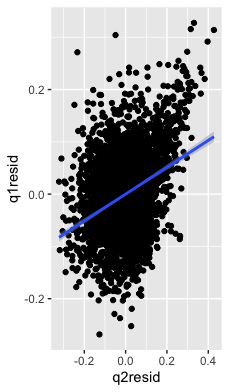
\includegraphics[scale=0.85]{plot_4.png}
		
		
		\item Write the prediction equation.
	\end{enumerate}
	
	\newpage	

\section*{Question 5}% (20 points)}
\noindent What if the incumbent's vote share is affected by both the president's popularity and the difference in spending between incumbent and challenger? 
	\begin{enumerate}
		\item Run a regression where the outcome variable is the incumbent's \texttt{voteshare} and the explanatory variables are \texttt{difflog} and \texttt{presvote}.	\vspace{5cm}
		
			\begin{lstlisting}[language=R]
			
			
			## 1. Run a regression where the outcome variable is the incumbent's 'voteshare' and 
# the explanatory variables are 'difflog' and 'presvote'


q5resid <- lm(voteshare ~ difflog + presvote, incumbents)
# summary(lm(voteshare ~ difflog + presvote, incumbents))
summary(q5resid)
			
		\end{lstlisting}
		
		\item Write the prediction equation.	\vspace{5cm}
		
		\begin{lstlisting}[language=R]
		
		## 2. Write the prediction equation

# (Intercept) 0.4486442
# difflog     0.0355431
# presvote    0.2568770
		
		\end{lstlisting}
		
		
		$\hat{y}$	= 0.4486442 + (0.0355431)x1 + (0.2568770)x2
		
		
		\item What is it in this output that is identical to the output in Question 4? Why do you think this is the case?%	\vspace{5cm}
	%	\item Reflect on your finding. Don't write anything. Just think about it.
	\end{enumerate}




\end{document}
